\newcommand{\ind}{\perp\!\!\!\!\perp}

\section{Bayes Net}
Two variables are independent ($X\ind Y$) iff $\forall x,y: P(x,y)=P(x)P(y)$ which is the same as $\forall x,y: P(x|y)=P(x)$ \\
$X$ is conditionally independent of $Y$ given $Z$ ($X\ind Y|Z$) iff $\forall x,y,z: P(x,y|z)=P(x|z)P(y|z)$ which is the same as $\forall x,y,z: P(x|z,y)=P(x|z)$ \\
Chain rule: $P(X_1,X_2,...,X_n)=P(X_1)P(X_2|X_1)P(X_3|X_1,X_2)...$ \\
In a Bayes Net, a node is a variable with a domain which can be assigned (observed) or unassigned (unobserved). Arcs encode conditional independence. \\
For a full assignment, calculate the probability by multiplying the conditionals: \\
$P(x_1,x_2,...,x_n)=\Pi^{n}_{i=1}P(x_i|\text{parents}(X_i))$ \\
\begin{figure}[H]
\centering
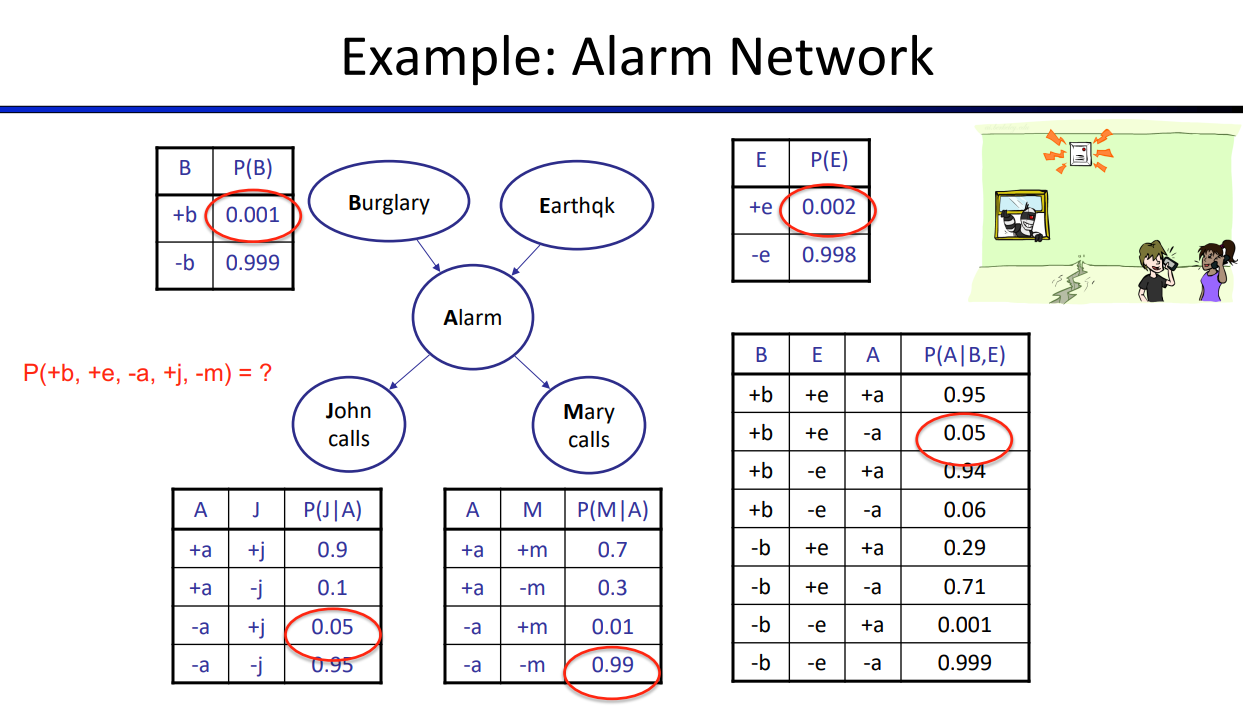
\includegraphics[width=\linewidth]{bayes-net-simple}
\end{figure}
Question: Are $X$ and $Y$ conditionally independent given evidence variables \{Z\}? \\
Consider all paths from $X$ to $Y$. If any of them are active, then they are conditionally \textbf{dependent}. \\
Equivalently, no active paths = conditional independence. \\
A path is active if each triple is active: \\
\begin{figure}[H]
\centering
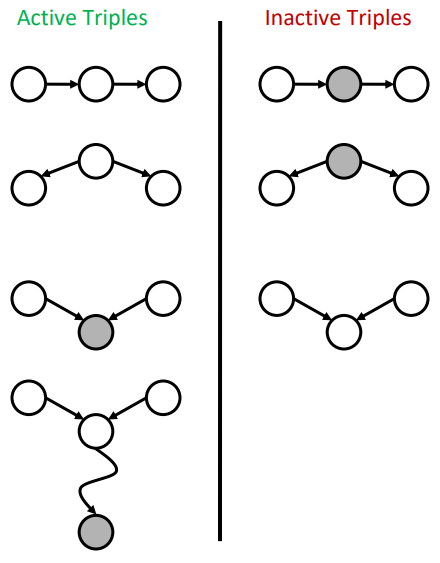
\includegraphics[width=\linewidth*2/5]{d-separation}
\end{figure}
\textbf{Inference by Enumeration}: Sum up the whole joint distribution before summing out the hidden variables. Simply select entries consistent with the evidence, sum out hidden variables $H$ to get joint of query and evidence, then normalize. It is the method used in the earlier example. \\
\textbf{Variable Elimination}: Interleave joining and marginalizing. Example below:
\begin{figure}[H]
\centering
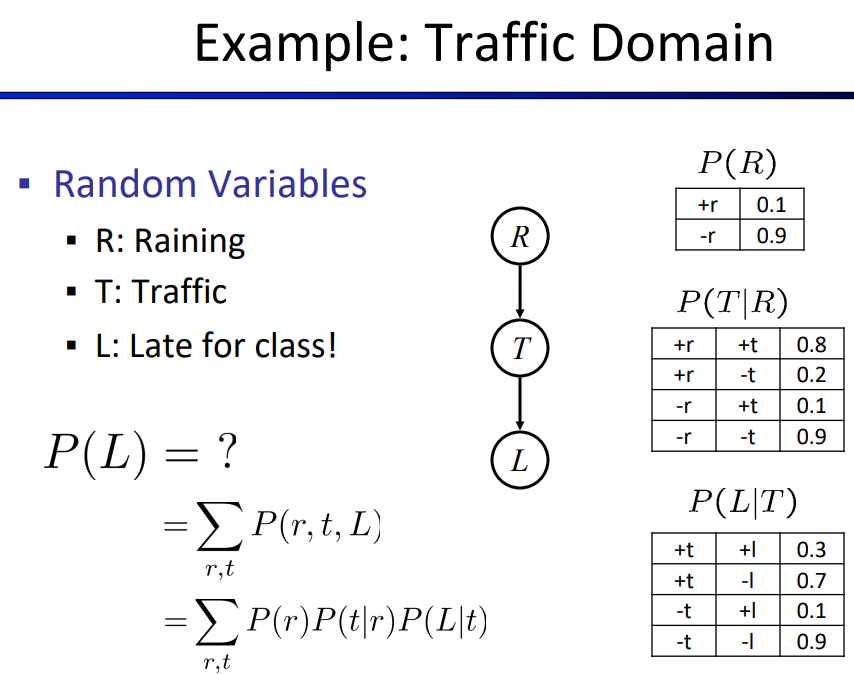
\includegraphics[width=\linewidth]{bayes-net-traffic-example-1}
\end{figure}
\begin{figure}[H]
\centering
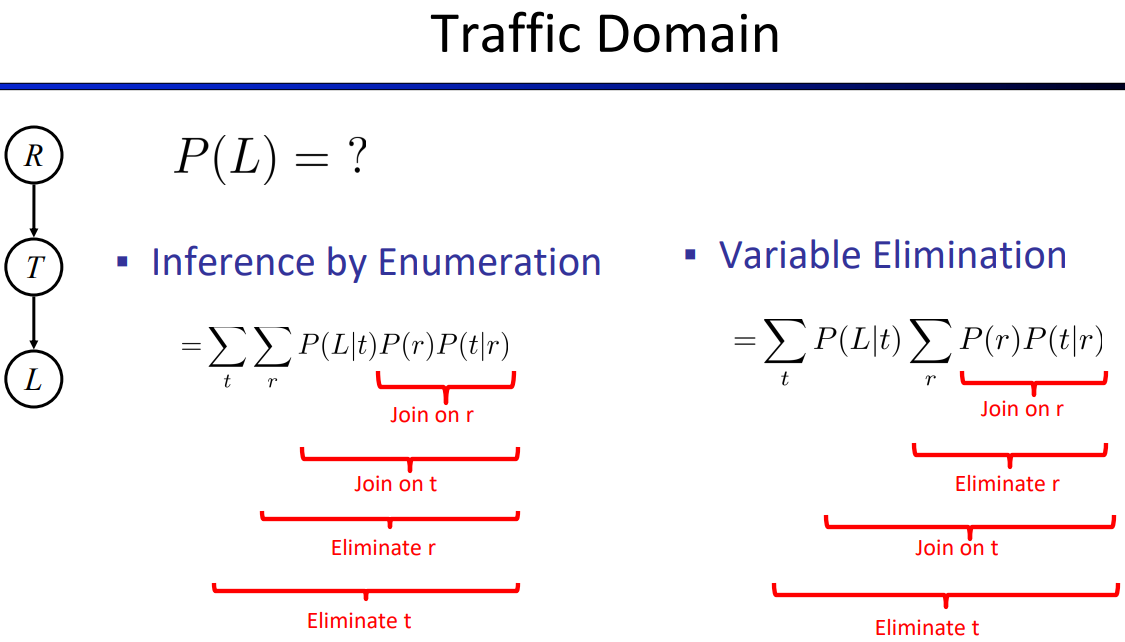
\includegraphics[width=\linewidth]{bayes-net-traffic-example-2}
\end{figure}
\begin{figure}[H]
\centering
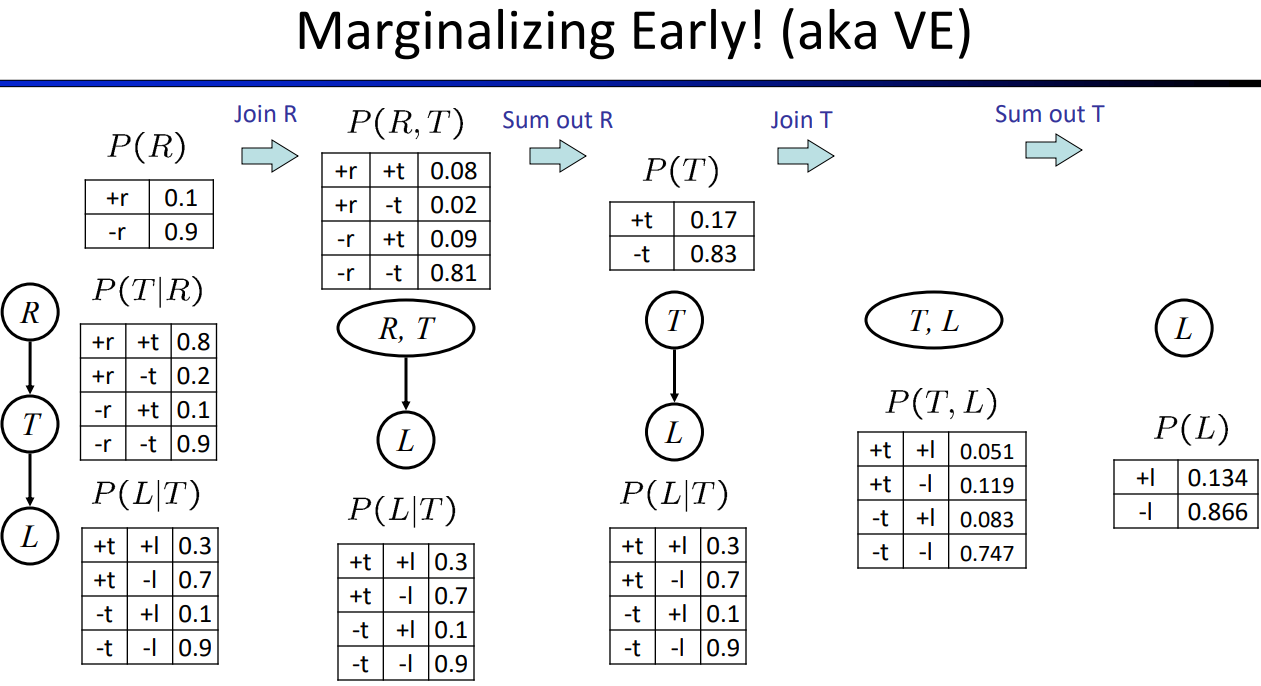
\includegraphics[width=\linewidth]{bayes-net-traffic-example-3}
\end{figure}
A way to do approximate inference with a Bayes' Net is with \textbf{sampling}; there are 4 types: \\
\textbf{Prior Sampling}: Samples random variables for each node according to its conditional probabilities; does not take evidence into account.
\begin{figure}[H]
\centering
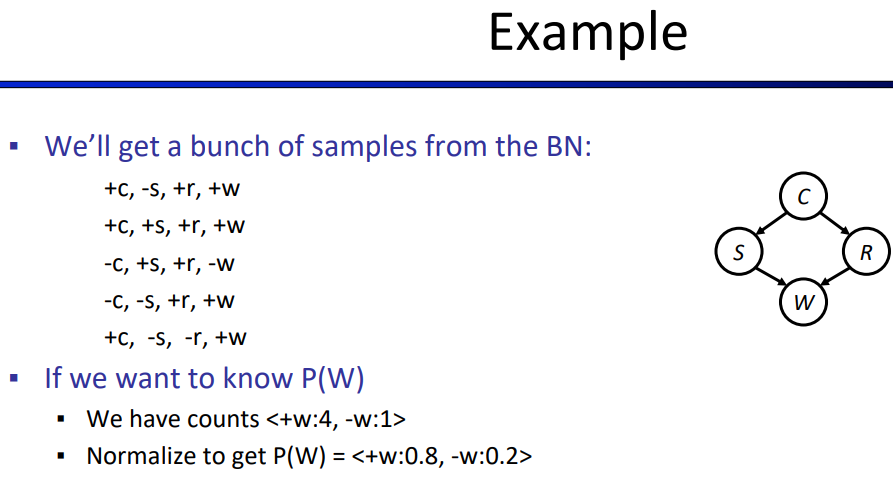
\includegraphics[width=\linewidth]{prior-sampling}
\end{figure}
\textbf{Rejection Sampling}: Same as prior sampling, except take evidence into account by throwing away samples that do not fit with evidence.
\begin{figure}[H]
\centering
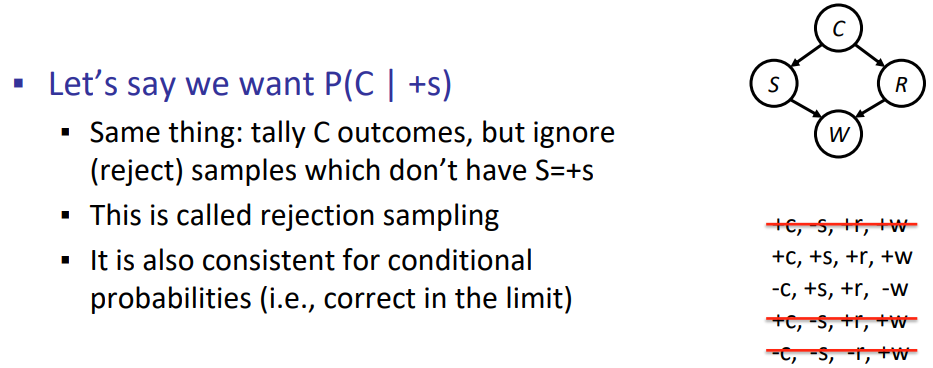
\includegraphics[width=\linewidth]{rejection-sampling}
\end{figure}
\textbf{Likelihood Weighting}: Instead of rejecting samples inconsistent with evidence, fix evidence variables and sample the rest. Then weight by probability of evidence given parents.
\begin{figure}[H]
\centering
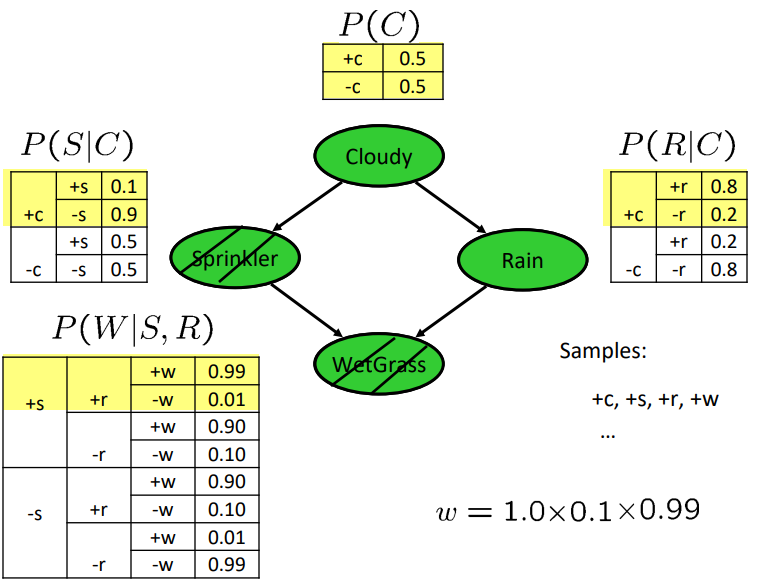
\includegraphics[width=\linewidth]{likelihood-weighting}
\end{figure}
\textbf{Gibbs Sampling}: Initialize variables randomly, then resample one variable at a time
\begin{figure}[H]
\centering
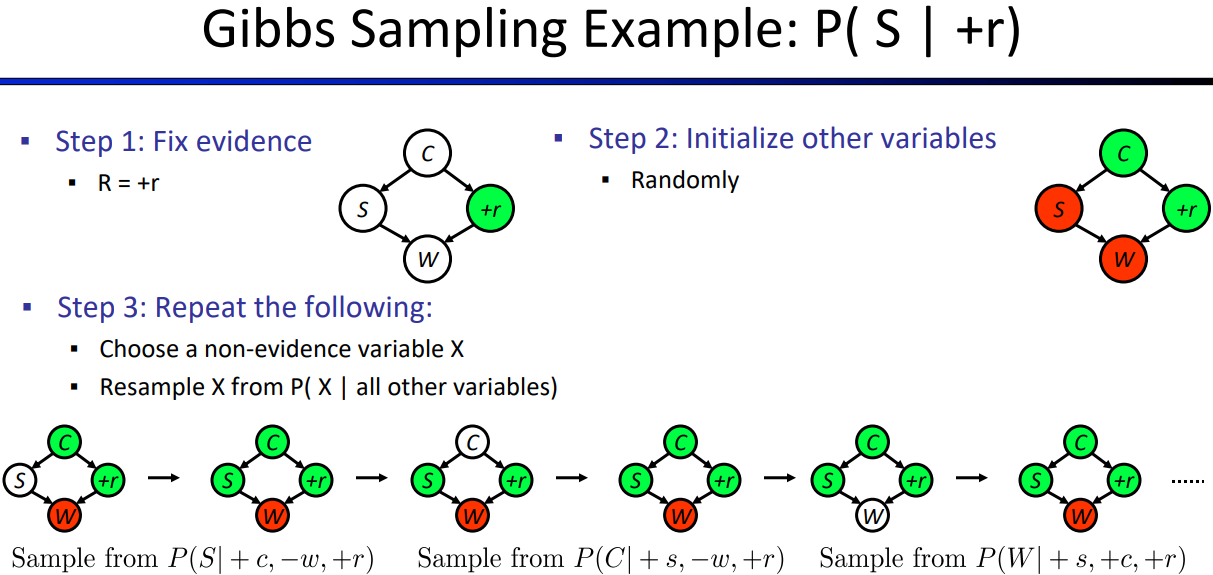
\includegraphics[width=\linewidth]{gibbs-sampling}
\end{figure}